\documentclass[10pt,a4paper]{article} % Prepara un documento con un font grande

% Adatta LaTeX alle convenzioni tipografiche italiane,
% e ridefinisce alcuni titoli in italiano, come "Capitolo" al posto di "Chapter",
% se il documento è in italiano
%\usepackage[italian]{babel}
%\usepackage[utf8]{inputenc} % Consente l'uso caratteri accentati italiani
%\usepackage{graphicx}		% Per le immagini
%\usepackage{gnuplot-lua-tikz}
%\usepackage[top=2.5cm, bottom=2cm, left=2cm, right=2cm]{geometry}

%\nonstopmode %non fermarti agli errori

%\usepackage{fancyhdr}
%\setlength{\headheight}{15.2pt}
%\pagestyle{fancy} % Solo le pagine normali, non i titoli nè la pagina iniziale


%%%%%%%%%%%%%%%%%%%%%%%%%%%%%%%%%%%%%%%%%%%%%%%%%%%%%%%%%%%%%%%%%%%%%%%%%%%%%%%%%%%%%%%%%

\usepackage{lipsum} % Package to generate dummy text throughout this template

%\usepackage[sc]{mathpazo} % Use the Palatino font
\usepackage{tgpagella} % TeX Gyre Pagella, versione migliorata di Palatino
%\usepackage{inconsolata}
\usepackage{textcomp}
\usepackage[scale=0.98,ttdefault]{AnonymousPro}

%%%%%
%\usepackage{Alegreya} %% Option 'black' gives heavier bold face 
%\renewcommand*\oldstylenums[1]{{\AlegreyaOsF #1}}

\usepackage[euler-digits,euler-hat-accent]{eulervm}
%%%%%%

\usepackage[T1]{fontenc} % Use 8-bit encoding that has 256 glyphs

\usepackage[utf8]{inputenc} % Consente l'uso caratteri accentati italiani
\linespread{1.06} % Line spacing - Palatino needs more space between lines
\usepackage{amsmath, amsthm, amssymb, amsfonts}
\usepackage[kerning,spacing]{microtype} % Slightly tweak font spacing for aesthetics

%%%%%%%%%%%%%%%%%%%%%%%%%%%%%%%%%%%%%%%%%%%%%
%Miei package
\usepackage[italian]{babel}
\usepackage{graphicx}		% Per le immagini
\usepackage{gnuplot-lua-tikz}
%%%%%%%%%%%%%%%%%%%%%%%%%%%%%%%%%%%%%%%%%%%%%
\usepackage[hmarginratio=1:1,top=32mm,columnsep=20pt]{geometry} % Document margins
\usepackage{multicol} % Used for the two-column layout of the document
\usepackage[hang, small,labelfont=bf,up,textfont=it,up]{caption} % Custom captions under/above floats in tables or figures
\usepackage{booktabs} % Horizontal rules in tables
\usepackage{float} % Required for tables and figures in the multi-column environment - they need to be placed in specific locations with the [H] (e.g. \begin{table}[H])
%\usepackage{hyperref} % For hyperlinks in the PDF
\usepackage{siunitx}

\usepackage{lettrine} % The lettrine is the first enlarged letter at the beginning of the text
\usepackage{paralist} % Used for the compactitem environment which makes bullet points with less space between them

\usepackage{abstract} % Allows abstract customization
\renewcommand{\abstractnamefont}{\normalfont\bfseries} % Set the "Abstract" text to bold
\renewcommand{\abstracttextfont}{\normalfont\small\itshape} % Set the abstract itself to small italic text

\usepackage{caption} % Per captions avanzate

\usepackage{listingsutf8} % Per includere codice sorgente meglio che con verbatim (e con caratteri non inglesi)
\lstset{ 
  %Preso anche questo da http://en.wikibooks.org/wiki/LaTeX/Source_Code_Listings
  %backgroundcolor=\color{white},   % choose the background color; you must add \usepackage{color} or \usepackage{xcolor}
  basicstyle=\footnotesize\ttfamily,        % the size of the fonts that are used for the code E MESSO IN MONOSPACE
  breakatwhitespace=false,         % sets if automatic breaks should only happen at whitespace
  breaklines=true,                 % sets automatic line breaking
  captionpos=b,                    % sets the caption-position to bottom
  %commentstyle=\color{mygreen},    % comment style
  %deletekeywords={...},            % if you want to delete keywords from the given language
  %escapeinside={\%*}{*)},          % if you want to add LaTeX within your code
  %extendedchars=true,              % lets you use non-ASCII characters; for 8-bits encodings only, does not work with UTF-8
  frame=l,                    % adds a frame around the code
				    %you can control the rules at the top, right, bottom, and left directly by using the four initial 
				    %letters for single rules and their upper case versions for double rules. http://mirror.hmc.edu/ctan/macros/latex/contrib/listings/listings.pdf
				    % Es frame frame=trBL ha doppia linea a sinistra e sotto, e singola a destra e sopra
  keepspaces=true,                 % keeps spaces in text, useful for keeping indentation of code (possibly needs columns=flexible)
  %keywordstyle=\color{blue},       % keyword style
  %language=Octave,                 % the language of the code
  %morekeywords={*,...},            % if you want to add more keywords to the set
  numbers=left,                    % where to put the line-numbers; possible values are (none, left, right)
  numbersep=5pt,                   % how far the line-numbers are from the code
  %numberstyle=\tiny\color{mygray}, % the style that is used for the line-numbers
  %rulecolor=\color{black},         % if not set, the frame-color may be changed on line-breaks within not-black text (e.g. comments (green here))
  showspaces=false,                % show spaces everywhere adding particular underscores; it overrides 'showstringspaces'
  showstringspaces=false,          % underline spaces within strings only
  showtabs=false,                  % show tabs within strings adding particular underscores
  stepnumber=1,                    % the step between two line-numbers. If it's 1, each line will be numbered
  %stringstyle=\color{mymauve},     % string literal style
  tabsize=2,                       % sets default tabsize to 2 spaces
  title=\lstname                   % show the filename of files included with \lstinputlisting; also try caption instead of title
}


\usepackage{titlesec} % Allows customization of titles
\renewcommand\thesection{\Roman{section}} % Roman numerals for the sections
\renewcommand\thesubsection{\Roman{subsection}} % Roman numerals for subsections
\titleformat{\section}[block]{\large\scshape\centering}{\thesection.}{1em}{} % Change the look of the section titles
\titleformat{\subsection}[block]{\large}{\thesubsection.}{1em}{} % Change the look of the section titles

\usepackage{fancyhdr} % Headers and footers
\pagestyle{fancy} % All pages have headers and footers
\fancyhead{} % Blank out the default header
\fancyfoot{} % Blank out the default footer
\fancyhead[C]{Running title $\bullet$ November 2012 $\bullet$ Vol. XXI, No. 1} % Custom header text
\fancyfoot[RO,LE]{\thepage} % Custom footer text



\DeclareGraphicsExtensions{.pdf, .png, .jpg} % Se due immagini hanno lo stesso nome sceglile secondo l'ordine di filetype qui
\graphicspath{ {./img/} }					 % Path delle immagini 

\title {\vspace{-2cm} \fontsize{60pt}{10pt}\selectfont\textsc{Pendolo a Torsione}}
\author{
\large
\textsc{Francesco Forcher}\\[2mm]
\normalsize Università di Padova, Facoltà di Fisica\\
\normalsize francesco.forcher@studenti.unipd.it\\
\normalsize Matricola: \texttt{1073458}\\
\and
\large
\textsc{Davide Chiappara}\\[2mm]
\normalsize Università di Padova, Facoltà di Fisica\\
\normalsize davide.chiappara@studenti.unipd.it\\
\normalsize Matricola: \texttt{1073458}\\
\and
\large
\textsc{Simone Frau}\\[2mm]
\normalsize Università di Padova, Facoltà di Fisica\\
\normalsize simone.forcher@studenti.unipd.it\\
\normalsize Matricola: \texttt{1073458}
}
\date{\today}

%%%%%%%%%%%%%%%%%%%%%%%%%%%%%%%%%%%%%%5%%%%%%%%%%%%%%%%%%%%%%%%%%%%%%%%%%%%%%%%%%%
\usepackage{float}
\usepackage{caption}
%\usepackage{multirow}
%\usepackage[top=3.6cm, bottom=1.5in, left=0.5in, right=0.5in]{geometry}


% I miei stili di float, con le righe
\floatstyle{ruled}
\newfloat{tabella}{H}{lop}
\floatname{tabella}{Tabella}

\floatstyle{ruled}
\newfloat{grafico}{H}{lop}
\floatname{grafico}{Grafico}
%%%%%%%%%%%%%%%%%%%%%%%%%%%%%%%%%%%%%%%%%%%%%%%%%%%%%%%%%%%%%%%%%%%%%5%%%%%%%%%%%%%



%////////////////////////////////////////////////////////////////////////////////////////////////////////////////////////////
%////////////////////////////////////////////////////////////////////////////////////////////////////////////////////////////
% Fine dei dati iniziali per il latex: il documento finale inizierà da qui
\begin{document}

\maketitle % Produce il titolo a partire dai comandi \title, \author e \date

\vspace{ \stretch{1} }
\begin{center}
	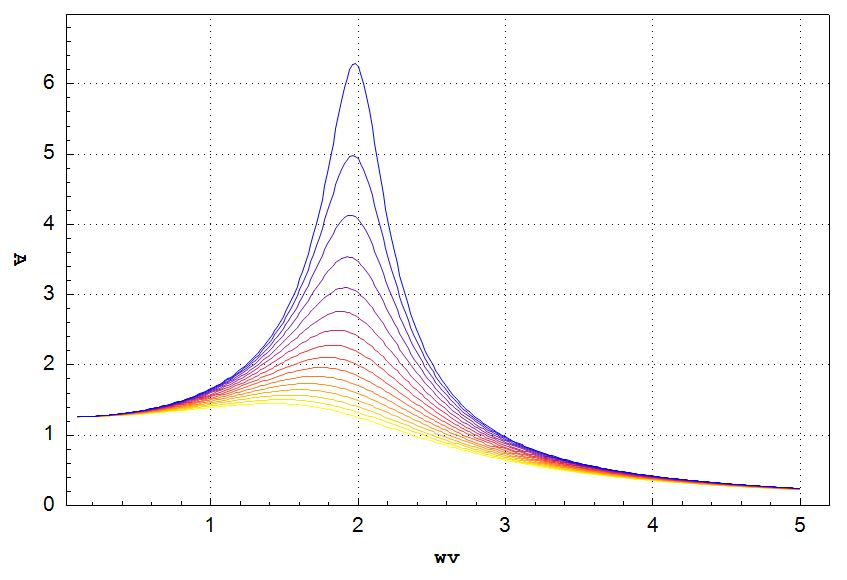
\includegraphics[width=0.8\textwidth]{risonanza}
\end{center}

\vspace{ \stretch{1} }
% Le varie sezioni
%\section{Obiettivi}
\begin{abstract}
	\noindent
	Obiettivo dell'esperienza è stato studiare il moto di un cilindro in acqua in risposta ad una forza periodica impressa
al clindro stesso da un motore elettrico attraverso un filo che permette la trasmissione di un momento torcente.
Dai campioni ricavati sperimentalmente si è indagato, in particolare, sulla curva di risonanza,  sulla frequenza di risonanza, sul coefficiente di smorzamento e sulla pulsazione propria del sistema.

\end{abstract}

\newpage



\microtypesetup{protrusion=false} % disables protrusion locally in the document
\tableofcontents % prints Table of Contents
\microtypesetup{protrusion=true} % enables protrusion

%\begin{multicols}{2}

\section{Apparato strumentale}
	L’apparato strumentale consiste in un cilindro in plexiglass al cui interno è posto un peso in acciaio di massa: $(115.5 /pm 0.1) g$
 e diametro: $(22.7 /pm 0.1)mm$ e altezza: $(34.0 /pm 0.1)mm$ collegato ad un filo di acciaio armonico, materiale dotato discrete
 capacità elastiche, ed immerso in un liquido. Il filo è inoltre collegato ad una piattaforma rotante azionata da un motore di
 diametro circa 8cm che, una volta azionato, induce un’oscillazione forzata del corpo formato dal filo più il pesetto. Il range delle
 frequenze alla quale il motore può essere indotto ad oscillare risulta compreso tra 0.8 e 1.2 Hz. Di suddetta oscillazione è
 possibile modificare il periodo e l’ampiezza. Il tutto viene controllato e registrato mediante l’interfaccia fornita da un computer.
 I dati vengono acquisiti in intervalli di 0.05 secondi permettendo una frequenza di rilevamento di 20 dati per secondo.
 L’interfaccia permette di visualizzare valori della frequenza, dell’ampiezza e della fase (espressa in gradi). Inoltre sono presenti
 diversi grafici che mostrano, in tempo reale, la curva di risonanza, il moto del pesetto, segnandone la posizione. Inoltre la
 presenza del pulsante offset permetteva di tarare l’apparato dopo ogni misurazione, al fine di limitare errori sistematici.




\section{Metodologia di misura}
	


%\newpage
\section{Presentazione dei dati}			
	\subsection{Tabelle}
	%\begin{multicols}{2}
	%\begin{tabella}
%	\centering
%	\input{./tabelle/dati_temperature.tex}
%	\caption{Temperature delle isoterme}
%	\label{tab:ad}
%\end{tabella}

	%\end{multicols}
	\clearpage
	\subsection{Grafici}
	%\begin{grafico}
%  \centering
%\begin{tikzpicture}[gnuplot]
%% generated with GNUPLOT 4.6p3 (Lua 5.1; terminal rev. 99, script rev. 100)
%% mar 27 mag 2014 18:54:53 CEST
\path (0.000,0.000) rectangle (12.500,8.750);
\gpcolor{color=gp lt color axes}
\gpsetlinetype{gp lt axes}
\gpsetlinewidth{1.00}
\draw[gp path] (1.196,0.763)--(11.947,0.763);
\gpcolor{color=gp lt color border}
\gpsetlinetype{gp lt border}
\draw[gp path] (1.196,0.763)--(1.376,0.763);
\draw[gp path] (11.947,0.763)--(11.767,0.763);
\node[gp node right] at (1.012,0.763) { 0.4};
\gpcolor{color=gp lt color axes}
\gpsetlinetype{gp lt axes}
\draw[gp path] (1.196,1.759)--(11.947,1.759);
\gpcolor{color=gp lt color border}
\gpsetlinetype{gp lt border}
\draw[gp path] (1.196,1.759)--(1.376,1.759);
\draw[gp path] (11.947,1.759)--(11.767,1.759);
\node[gp node right] at (1.012,1.759) { 0.6};
\gpcolor{color=gp lt color axes}
\gpsetlinetype{gp lt axes}
\draw[gp path] (1.196,2.755)--(11.947,2.755);
\gpcolor{color=gp lt color border}
\gpsetlinetype{gp lt border}
\draw[gp path] (1.196,2.755)--(1.376,2.755);
\draw[gp path] (11.947,2.755)--(11.767,2.755);
\node[gp node right] at (1.012,2.755) { 0.8};
\gpcolor{color=gp lt color axes}
\gpsetlinetype{gp lt axes}
\draw[gp path] (1.196,3.751)--(11.947,3.751);
\gpcolor{color=gp lt color border}
\gpsetlinetype{gp lt border}
\draw[gp path] (1.196,3.751)--(1.376,3.751);
\draw[gp path] (11.947,3.751)--(11.767,3.751);
\node[gp node right] at (1.012,3.751) { 1};
\gpcolor{color=gp lt color axes}
\gpsetlinetype{gp lt axes}
\draw[gp path] (1.196,4.748)--(11.947,4.748);
\gpcolor{color=gp lt color border}
\gpsetlinetype{gp lt border}
\draw[gp path] (1.196,4.748)--(1.376,4.748);
\draw[gp path] (11.947,4.748)--(11.767,4.748);
\node[gp node right] at (1.012,4.748) { 1.2};
\gpcolor{color=gp lt color axes}
\gpsetlinetype{gp lt axes}
\draw[gp path] (1.196,5.744)--(11.947,5.744);
\gpcolor{color=gp lt color border}
\gpsetlinetype{gp lt border}
\draw[gp path] (1.196,5.744)--(1.376,5.744);
\draw[gp path] (11.947,5.744)--(11.767,5.744);
\node[gp node right] at (1.012,5.744) { 1.4};
\gpcolor{color=gp lt color axes}
\gpsetlinetype{gp lt axes}
\draw[gp path] (1.196,6.740)--(11.947,6.740);
\gpcolor{color=gp lt color border}
\gpsetlinetype{gp lt border}
\draw[gp path] (1.196,6.740)--(1.376,6.740);
\draw[gp path] (11.947,6.740)--(11.767,6.740);
\node[gp node right] at (1.012,6.740) { 1.6};
\gpcolor{color=gp lt color axes}
\gpsetlinetype{gp lt axes}
\draw[gp path] (1.196,7.736)--(4.591,7.736);
\draw[gp path] (11.763,7.736)--(11.947,7.736);
\gpcolor{color=gp lt color border}
\gpsetlinetype{gp lt border}
\draw[gp path] (1.196,7.736)--(1.376,7.736);
\draw[gp path] (11.947,7.736)--(11.767,7.736);
\node[gp node right] at (1.012,7.736) { 1.8};
\gpcolor{color=gp lt color axes}
\gpsetlinetype{gp lt axes}
\draw[gp path] (1.514,0.616)--(1.514,8.381);
\gpcolor{color=gp lt color border}
\gpsetlinetype{gp lt border}
\draw[gp path] (1.514,0.616)--(1.514,0.796);
\draw[gp path] (1.514,8.381)--(1.514,8.201);
\node[gp node center] at (1.514,0.308) { 0.02};
\gpcolor{color=gp lt color axes}
\gpsetlinetype{gp lt axes}
\draw[gp path] (2.779,0.616)--(2.779,8.381);
\gpcolor{color=gp lt color border}
\gpsetlinetype{gp lt border}
\draw[gp path] (2.779,0.616)--(2.779,0.796);
\draw[gp path] (2.779,8.381)--(2.779,8.201);
\node[gp node center] at (2.779,0.308) { 0.04};
\gpcolor{color=gp lt color axes}
\gpsetlinetype{gp lt axes}
\draw[gp path] (4.043,0.616)--(4.043,8.381);
\gpcolor{color=gp lt color border}
\gpsetlinetype{gp lt border}
\draw[gp path] (4.043,0.616)--(4.043,0.796);
\draw[gp path] (4.043,8.381)--(4.043,8.201);
\node[gp node center] at (4.043,0.308) { 0.06};
\gpcolor{color=gp lt color axes}
\gpsetlinetype{gp lt axes}
\draw[gp path] (5.307,0.616)--(5.307,6.969);
\draw[gp path] (5.307,8.201)--(5.307,8.381);
\gpcolor{color=gp lt color border}
\gpsetlinetype{gp lt border}
\draw[gp path] (5.307,0.616)--(5.307,0.796);
\draw[gp path] (5.307,8.381)--(5.307,8.201);
\node[gp node center] at (5.307,0.308) { 0.08};
\gpcolor{color=gp lt color axes}
\gpsetlinetype{gp lt axes}
\draw[gp path] (6.571,0.616)--(6.571,6.969);
\draw[gp path] (6.571,8.201)--(6.571,8.381);
\gpcolor{color=gp lt color border}
\gpsetlinetype{gp lt border}
\draw[gp path] (6.571,0.616)--(6.571,0.796);
\draw[gp path] (6.571,8.381)--(6.571,8.201);
\node[gp node center] at (6.571,0.308) { 0.1};
\gpcolor{color=gp lt color axes}
\gpsetlinetype{gp lt axes}
\draw[gp path] (7.836,0.616)--(7.836,6.969);
\draw[gp path] (7.836,8.201)--(7.836,8.381);
\gpcolor{color=gp lt color border}
\gpsetlinetype{gp lt border}
\draw[gp path] (7.836,0.616)--(7.836,0.796);
\draw[gp path] (7.836,8.381)--(7.836,8.201);
\node[gp node center] at (7.836,0.308) { 0.12};
\gpcolor{color=gp lt color axes}
\gpsetlinetype{gp lt axes}
\draw[gp path] (9.100,0.616)--(9.100,6.969);
\draw[gp path] (9.100,8.201)--(9.100,8.381);
\gpcolor{color=gp lt color border}
\gpsetlinetype{gp lt border}
\draw[gp path] (9.100,0.616)--(9.100,0.796);
\draw[gp path] (9.100,8.381)--(9.100,8.201);
\node[gp node center] at (9.100,0.308) { 0.14};
\gpcolor{color=gp lt color axes}
\gpsetlinetype{gp lt axes}
\draw[gp path] (10.364,0.616)--(10.364,6.969);
\draw[gp path] (10.364,8.201)--(10.364,8.381);
\gpcolor{color=gp lt color border}
\gpsetlinetype{gp lt border}
\draw[gp path] (10.364,0.616)--(10.364,0.796);
\draw[gp path] (10.364,8.381)--(10.364,8.201);
\node[gp node center] at (10.364,0.308) { 0.16};
\gpcolor{color=gp lt color axes}
\gpsetlinetype{gp lt axes}
\draw[gp path] (11.629,0.616)--(11.629,6.969);
\draw[gp path] (11.629,8.201)--(11.629,8.381);
\gpcolor{color=gp lt color border}
\gpsetlinetype{gp lt border}
\draw[gp path] (11.629,0.616)--(11.629,0.796);
\draw[gp path] (11.629,8.381)--(11.629,8.201);
\node[gp node center] at (11.629,0.308) { 0.18};
\draw[gp path] (1.196,8.381)--(1.196,0.616)--(11.947,0.616)--(11.947,8.381)--cycle;
\node[gp node right] at (10.479,8.047) {'TEST_isobara2' using (1.0/$3):($1)};
\gpcolor{color=gp lt color 0}
\gpsetlinetype{gp lt plot 0}
\draw[gp path] (10.663,8.047)--(11.579,8.047);
\draw[gp path] (7.749,5.943)--(4.960,5.943)--(4.957,5.943)--(6.778,5.943)--(5.876,5.943)%
  --(6.139,5.943)--(6.691,5.943)--(6.697,5.943)--(6.690,5.943)--(5.705,5.943)--(6.665,5.943)%
  --(6.909,5.943)--(6.927,5.943)--(6.906,5.943)--(6.915,5.943)--(6.964,5.943)--(6.958,5.943)%
  --(6.088,5.943)--(6.091,5.943)--(8.074,5.943)--(8.073,5.943)--(8.072,5.943)--(8.073,5.943)%
  --(6.482,5.943)--(6.488,5.943)--(7.433,5.943)--(7.757,5.948)--(4.965,5.948)--(6.797,5.948)%
  --(6.793,5.948)--(6.783,5.948)--(6.804,5.948)--(6.801,5.948)--(5.879,5.948)--(5.881,5.948)%
  --(6.144,5.948)--(5.706,5.948)--(5.705,5.948)--(6.672,5.948)--(6.680,5.948)--(6.942,5.948)%
  --(6.959,5.948)--(6.970,5.948)--(6.091,5.948)--(8.079,5.948)--(8.096,5.948)--(8.084,5.948)%
  --(6.489,5.948)--(7.455,5.948)--(7.447,5.948)--(7.478,5.948)--(7.463,5.948)--(4.970,5.953)%
  --(6.809,5.953)--(5.885,5.953)--(6.150,5.953)--(6.702,5.953)--(5.711,5.953)--(6.966,5.953)%
  --(6.971,5.953)--(6.983,5.953)--(6.099,5.953)--(8.096,5.953)--(6.493,5.953)--(7.477,5.953)%
  --(4.975,5.958)--(5.892,5.958)--(5.887,5.958)--(6.155,5.958)--(6.706,5.958)--(5.717,5.958)%
  --(5.720,5.958)--(6.982,5.958)--(6.998,5.958)--(6.120,5.958)--(6.108,5.958)--(8.109,5.958)%
  --(8.105,5.958)--(7.477,5.958);
\gpcolor{color=gp lt color border}
\node[gp node right] at (10.479,7.739) {'TEST_isobara1' using (1.0/$3):($1)};
\gpcolor{color=gp lt color 1}
\gpsetpointsize{4.00}
\gppoint{gp mark 2}{(4.687,4.499)}
\gppoint{gp mark 2}{(4.644,4.499)}
\gppoint{gp mark 2}{(4.640,4.499)}
\gppoint{gp mark 2}{(4.160,4.499)}
\gppoint{gp mark 2}{(4.155,4.499)}
\gppoint{gp mark 2}{(4.159,4.499)}
\gppoint{gp mark 2}{(5.096,4.499)}
\gppoint{gp mark 2}{(5.095,4.499)}
\gppoint{gp mark 2}{(5.095,4.499)}
\gppoint{gp mark 2}{(4.269,4.499)}
\gppoint{gp mark 2}{(4.270,4.499)}
\gppoint{gp mark 2}{(5.253,4.499)}
\gppoint{gp mark 2}{(4.545,4.499)}
\gppoint{gp mark 2}{(3.835,4.499)}
\gppoint{gp mark 2}{(3.834,4.499)}
\gppoint{gp mark 2}{(3.832,4.499)}
\gppoint{gp mark 2}{(6.466,4.499)}
\gppoint{gp mark 2}{(6.462,4.499)}
\gppoint{gp mark 2}{(6.460,4.499)}
\gppoint{gp mark 2}{(4.895,4.499)}
\gppoint{gp mark 2}{(5.248,4.499)}
\gppoint{gp mark 2}{(5.258,4.499)}
\gppoint{gp mark 2}{(5.238,4.499)}
\gppoint{gp mark 2}{(5.242,4.499)}
\gppoint{gp mark 2}{(3.483,4.503)}
\gppoint{gp mark 2}{(4.691,4.503)}
\gppoint{gp mark 2}{(4.163,4.503)}
\gppoint{gp mark 2}{(4.165,4.503)}
\gppoint{gp mark 2}{(5.096,4.503)}
\gppoint{gp mark 2}{(4.274,4.503)}
\gppoint{gp mark 2}{(4.786,4.503)}
\gppoint{gp mark 2}{(4.553,4.503)}
\gppoint{gp mark 2}{(3.837,4.503)}
\gppoint{gp mark 2}{(3.836,4.503)}
\gppoint{gp mark 2}{(6.463,4.503)}
\gppoint{gp mark 2}{(6.463,4.503)}
\gppoint{gp mark 2}{(4.902,4.503)}
\gppoint{gp mark 2}{(6.052,4.508)}
\gppoint{gp mark 2}{(3.485,4.508)}
\gppoint{gp mark 2}{(4.695,4.508)}
\gppoint{gp mark 2}{(4.651,4.508)}
\gppoint{gp mark 2}{(4.650,4.508)}
\gppoint{gp mark 2}{(4.649,4.508)}
\gppoint{gp mark 2}{(4.170,4.508)}
\gppoint{gp mark 2}{(4.166,4.508)}
\gppoint{gp mark 2}{(5.100,4.508)}
\gppoint{gp mark 2}{(5.099,4.508)}
\gppoint{gp mark 2}{(5.099,4.508)}
\gppoint{gp mark 2}{(5.101,4.508)}
\gppoint{gp mark 2}{(5.100,4.508)}
\gppoint{gp mark 2}{(4.290,4.508)}
\gppoint{gp mark 2}{(4.283,4.508)}
\gppoint{gp mark 2}{(4.280,4.508)}
\gppoint{gp mark 2}{(4.287,4.508)}
\gppoint{gp mark 2}{(5.258,4.508)}
\gppoint{gp mark 2}{(5.257,4.508)}
\gppoint{gp mark 2}{(4.554,4.508)}
\gppoint{gp mark 2}{(3.838,4.508)}
\gppoint{gp mark 2}{(6.464,4.508)}
\gppoint{gp mark 2}{(6.465,4.508)}
\gppoint{gp mark 2}{(4.901,4.508)}
\gppoint{gp mark 2}{(5.267,4.508)}
\gppoint{gp mark 2}{(5.259,4.508)}
\gppoint{gp mark 2}{(6.054,4.513)}
\gppoint{gp mark 2}{(3.511,4.513)}
\gppoint{gp mark 2}{(3.504,4.513)}
\gppoint{gp mark 2}{(3.500,4.513)}
\gppoint{gp mark 2}{(3.491,4.513)}
\gppoint{gp mark 2}{(3.498,4.513)}
\gppoint{gp mark 2}{(3.493,4.513)}
\gppoint{gp mark 2}{(3.505,4.513)}
\gppoint{gp mark 2}{(3.501,4.513)}
\gppoint{gp mark 2}{(3.495,4.513)}
\gppoint{gp mark 2}{(3.488,4.513)}
\gppoint{gp mark 2}{(3.503,4.513)}
\gppoint{gp mark 2}{(4.699,4.513)}
\gppoint{gp mark 2}{(4.725,4.513)}
\gppoint{gp mark 2}{(4.716,4.513)}
\gppoint{gp mark 2}{(4.713,4.513)}
\gppoint{gp mark 2}{(4.729,4.513)}
\gppoint{gp mark 2}{(4.711,4.513)}
\gppoint{gp mark 2}{(4.707,4.513)}
\gppoint{gp mark 2}{(4.705,4.513)}
\gppoint{gp mark 2}{(4.702,4.513)}
\gppoint{gp mark 2}{(4.652,4.513)}
\gppoint{gp mark 2}{(4.652,4.513)}
\gppoint{gp mark 2}{(4.651,4.513)}
\gppoint{gp mark 2}{(4.175,4.513)}
\gppoint{gp mark 2}{(4.173,4.513)}
\gppoint{gp mark 2}{(5.103,4.513)}
\gppoint{gp mark 2}{(4.293,4.513)}
\gppoint{gp mark 2}{(4.297,4.513)}
\gppoint{gp mark 2}{(5.261,4.513)}
\gppoint{gp mark 2}{(4.789,4.513)}
\gppoint{gp mark 2}{(4.557,4.513)}
\gppoint{gp mark 2}{(3.841,4.513)}
\gppoint{gp mark 2}{(3.841,4.513)}
\gppoint{gp mark 2}{(3.841,4.513)}
\gppoint{gp mark 2}{(6.465,4.513)}
\gppoint{gp mark 2}{(6.465,4.513)}
\gppoint{gp mark 2}{(5.273,4.513)}
\gppoint{gp mark 2}{(11.121,7.739)}
\gpcolor{color=gp lt color border}
\node[gp node right] at (10.479,7.431) {'TEST_isobara3' using (1.0/$3):($1)};
\gpcolor{color=gp lt color 2}
\gppoint{gp mark 3}{(3.911,2.257)}
\gppoint{gp mark 3}{(4.591,2.257)}
\gppoint{gp mark 3}{(4.594,2.257)}
\gppoint{gp mark 3}{(3.430,2.257)}
\gppoint{gp mark 3}{(3.431,2.257)}
\gppoint{gp mark 3}{(3.430,2.257)}
\gppoint{gp mark 3}{(3.457,2.257)}
\gppoint{gp mark 3}{(3.471,2.257)}
\gppoint{gp mark 3}{(3.971,2.257)}
\gppoint{gp mark 3}{(3.892,2.257)}
\gppoint{gp mark 3}{(3.296,2.257)}
\gppoint{gp mark 3}{(3.297,2.257)}
\gppoint{gp mark 3}{(3.713,2.257)}
\gppoint{gp mark 3}{(3.712,2.257)}
\gppoint{gp mark 3}{(3.710,2.257)}
\gppoint{gp mark 3}{(3.488,2.257)}
\gppoint{gp mark 3}{(4.932,2.257)}
\gppoint{gp mark 3}{(3.945,2.257)}
\gppoint{gp mark 3}{(3.946,2.257)}
\gppoint{gp mark 3}{(3.942,2.257)}
\gppoint{gp mark 3}{(3.947,2.257)}
\gppoint{gp mark 3}{(3.946,2.257)}
\gppoint{gp mark 3}{(3.455,2.257)}
\gppoint{gp mark 3}{(3.594,2.257)}
\gppoint{gp mark 3}{(3.910,2.262)}
\gppoint{gp mark 3}{(4.597,2.262)}
\gppoint{gp mark 3}{(3.433,2.262)}
\gppoint{gp mark 3}{(3.433,2.262)}
\gppoint{gp mark 3}{(3.458,2.262)}
\gppoint{gp mark 3}{(3.459,2.262)}
\gppoint{gp mark 3}{(3.470,2.262)}
\gppoint{gp mark 3}{(3.468,2.262)}
\gppoint{gp mark 3}{(3.468,2.262)}
\gppoint{gp mark 3}{(3.975,2.262)}
\gppoint{gp mark 3}{(3.896,2.262)}
\gppoint{gp mark 3}{(3.295,2.262)}
\gppoint{gp mark 3}{(3.718,2.262)}
\gppoint{gp mark 3}{(3.722,2.262)}
\gppoint{gp mark 3}{(3.720,2.262)}
\gppoint{gp mark 3}{(3.716,2.262)}
\gppoint{gp mark 3}{(3.719,2.262)}
\gppoint{gp mark 3}{(3.716,2.262)}
\gppoint{gp mark 3}{(3.489,2.262)}
\gppoint{gp mark 3}{(4.938,2.262)}
\gppoint{gp mark 3}{(4.945,2.262)}
\gppoint{gp mark 3}{(3.940,2.262)}
\gppoint{gp mark 3}{(3.938,2.262)}
\gppoint{gp mark 3}{(3.936,2.262)}
\gppoint{gp mark 3}{(3.938,2.262)}
\gppoint{gp mark 3}{(3.910,2.267)}
\gppoint{gp mark 3}{(4.597,2.267)}
\gppoint{gp mark 3}{(3.434,2.267)}
\gppoint{gp mark 3}{(3.465,2.267)}
\gppoint{gp mark 3}{(3.460,2.267)}
\gppoint{gp mark 3}{(3.459,2.267)}
\gppoint{gp mark 3}{(3.462,2.267)}
\gppoint{gp mark 3}{(3.467,2.267)}
\gppoint{gp mark 3}{(3.463,2.267)}
\gppoint{gp mark 3}{(3.465,2.267)}
\gppoint{gp mark 3}{(3.976,2.267)}
\gppoint{gp mark 3}{(3.464,2.267)}
\gppoint{gp mark 3}{(3.976,2.267)}
\gppoint{gp mark 3}{(3.295,2.267)}
\gppoint{gp mark 3}{(3.293,2.267)}
\gppoint{gp mark 3}{(3.724,2.267)}
\gppoint{gp mark 3}{(3.491,2.267)}
\gppoint{gp mark 3}{(3.500,2.267)}
\gppoint{gp mark 3}{(4.943,2.267)}
\gppoint{gp mark 3}{(3.934,2.267)}
\gppoint{gp mark 3}{(3.931,2.267)}
\gppoint{gp mark 3}{(3.933,2.267)}
\gppoint{gp mark 3}{(3.931,2.267)}
\gppoint{gp mark 3}{(3.936,2.267)}
\gppoint{gp mark 3}{(3.930,2.267)}
\gppoint{gp mark 3}{(3.457,2.267)}
\gppoint{gp mark 3}{(3.596,2.267)}
\gppoint{gp mark 3}{(3.593,2.267)}
\gppoint{gp mark 3}{(3.909,2.272)}
\gppoint{gp mark 3}{(3.907,2.272)}
\gppoint{gp mark 3}{(3.905,2.272)}
\gppoint{gp mark 3}{(4.599,2.272)}
\gppoint{gp mark 3}{(4.602,2.272)}
\gppoint{gp mark 3}{(3.435,2.272)}
\gppoint{gp mark 3}{(3.466,2.272)}
\gppoint{gp mark 3}{(3.465,2.272)}
\gppoint{gp mark 3}{(3.463,2.272)}
\gppoint{gp mark 3}{(3.976,2.272)}
\gppoint{gp mark 3}{(3.903,2.272)}
\gppoint{gp mark 3}{(3.293,2.272)}
\gppoint{gp mark 3}{(3.725,2.272)}
\gppoint{gp mark 3}{(3.506,2.272)}
\gppoint{gp mark 3}{(3.498,2.272)}
\gppoint{gp mark 3}{(3.495,2.272)}
\gppoint{gp mark 3}{(3.503,2.272)}
\gppoint{gp mark 3}{(3.494,2.272)}
\gppoint{gp mark 3}{(3.504,2.272)}
\gppoint{gp mark 3}{(3.497,2.272)}
\gppoint{gp mark 3}{(4.944,2.272)}
\gppoint{gp mark 3}{(3.929,2.272)}
\gppoint{gp mark 3}{(3.928,2.272)}
\gppoint{gp mark 3}{(3.460,2.272)}
\gppoint{gp mark 3}{(3.599,2.272)}
\gppoint{gp mark 3}{(11.121,7.431)}
\gpcolor{color=gp lt color border}
\node[gp node right] at (10.479,7.123) {'TEST_isobara4' using (1.0/$3):($1)};
\gpcolor{color=gp lt color 3}
\gppoint{gp mark 4}{(9.770,7.138)}
\gppoint{gp mark 4}{(8.132,7.138)}
\gppoint{gp mark 4}{(8.137,7.138)}
\gppoint{gp mark 4}{(9.320,7.138)}
\gppoint{gp mark 4}{(9.335,7.138)}
\gppoint{gp mark 4}{(8.202,7.138)}
\gppoint{gp mark 4}{(8.217,7.138)}
\gppoint{gp mark 4}{(8.193,7.138)}
\gppoint{gp mark 4}{(9.846,7.138)}
\gppoint{gp mark 4}{(9.866,7.138)}
\gppoint{gp mark 4}{(9.971,7.138)}
\gppoint{gp mark 4}{(9.947,7.138)}
\gppoint{gp mark 4}{(7.887,7.138)}
\gppoint{gp mark 4}{(9.773,7.143)}
\gppoint{gp mark 4}{(8.144,7.143)}
\gppoint{gp mark 4}{(8.152,7.143)}
\gppoint{gp mark 4}{(9.352,7.143)}
\gppoint{gp mark 4}{(9.974,7.143)}
\gppoint{gp mark 4}{(9.946,7.143)}
\gppoint{gp mark 4}{(9.898,7.143)}
\gppoint{gp mark 4}{(9.998,7.143)}
\gppoint{gp mark 4}{(9.984,7.143)}
\gppoint{gp mark 4}{(9.928,7.143)}
\gppoint{gp mark 4}{(7.887,7.143)}
\gppoint{gp mark 4}{(8.756,7.143)}
\gppoint{gp mark 4}{(9.802,7.148)}
\gppoint{gp mark 4}{(9.805,7.148)}
\gppoint{gp mark 4}{(9.788,7.148)}
\gppoint{gp mark 4}{(9.782,7.148)}
\gppoint{gp mark 4}{(9.822,7.148)}
\gppoint{gp mark 4}{(8.169,7.148)}
\gppoint{gp mark 4}{(8.162,7.148)}
\gppoint{gp mark 4}{(8.176,7.148)}
\gppoint{gp mark 4}{(9.368,7.148)}
\gppoint{gp mark 4}{(9.380,7.148)}
\gppoint{gp mark 4}{(9.367,7.148)}
\gppoint{gp mark 4}{(8.228,7.148)}
\gppoint{gp mark 4}{(8.230,7.148)}
\gppoint{gp mark 4}{(8.224,7.148)}
\gppoint{gp mark 4}{(10.024,7.148)}
\gppoint{gp mark 4}{(9.993,7.148)}
\gppoint{gp mark 4}{(10.002,7.148)}
\gppoint{gp mark 4}{(10.014,7.148)}
\gppoint{gp mark 4}{(9.998,7.148)}
\gppoint{gp mark 4}{(10.030,7.148)}
\gppoint{gp mark 4}{(7.899,7.148)}
\gppoint{gp mark 4}{(7.894,7.148)}
\gppoint{gp mark 4}{(7.905,7.148)}
\gppoint{gp mark 4}{(8.767,7.148)}
\gppoint{gp mark 4}{(9.847,7.153)}
\gppoint{gp mark 4}{(9.840,7.153)}
\gppoint{gp mark 4}{(9.834,7.153)}
\gppoint{gp mark 4}{(8.192,7.153)}
\gppoint{gp mark 4}{(8.178,7.153)}
\gppoint{gp mark 4}{(8.181,7.153)}
\gppoint{gp mark 4}{(9.397,7.153)}
\gppoint{gp mark 4}{(9.386,7.153)}
\gppoint{gp mark 4}{(9.384,7.153)}
\gppoint{gp mark 4}{(10.068,7.153)}
\gppoint{gp mark 4}{(10.100,7.153)}
\gppoint{gp mark 4}{(10.077,7.153)}
\gppoint{gp mark 4}{(10.065,7.153)}
\gppoint{gp mark 4}{(7.936,7.153)}
\gppoint{gp mark 4}{(7.918,7.153)}
\gppoint{gp mark 4}{(8.776,7.153)}
\gppoint{gp mark 4}{(11.121,7.123)}
\gpcolor{color=gp lt color border}
\gpsetlinetype{gp lt border}
\draw[gp path] (1.196,8.381)--(1.196,0.616)--(11.947,0.616)--(11.947,8.381)--cycle;
%% coordinates of the plot area
\gpdefrectangularnode{gp plot 1}{\pgfpoint{1.196cm}{0.616cm}}{\pgfpoint{11.947cm}{8.381cm}}
\end{tikzpicture}
%% gnuplot variables

%\caption{Alcune isobare estratte dai grafici}
%\label{img:isob}
%\end{grafico}
	
\clearpage
\section{Analisi dei dati}
	Come detto nella descrizione dell'apparato strumentale, il tasso di rilevamento dei dati è di 20 al secondo. Questo corrisponde a una
frequenza di campionamento di 20 Hertz, di molto superiore al 
Nyquist rate necessario per il pendolo (il doppio della massima frequenza
necessaria), dato che come verificabile a vista ha una frequenza dell'ordine di 1 Hz. 
Non ci sono quindi problemi di aliasing e sottocampionamento.
Per quanto riguarda l'offset, è stato rifatta la calibrazione prima di ogni presa dati (inizio giornata) e si può vedere che era
 calibrato da un'evidente simmetria rispetto all'asse delle ascisse.
Per il calcolo dei massimi è stato utilizzato un programma che riconoscesse i punti di massimo e minimo approssimando
la funzione come una parabola in un intorno dei dati "stazionari" (dati massimi e minimi locali) usando il dato precedente e il successivo,
vincolando la parabola a passare per questi 3 punti e trovandone il vertice. L'errore legato all'utilizzo
 di questa approssimazione è $o(x^3)$, come noto dallo sviluppo di Taylor delle funzioni goniometriche.

Per una stima delle ampiezze legate alle frequenze di oscillazione sono stati presi i valori medi...

Una stima della pulsazione di risonanza è stata fatta con un processo di esplorazione iniziale che ha permesso, attraverso
il metodo di bisezione, di concentrarsi sull'area nella quale l'ampiezza era più alta. Il valore finale trovato risulta di...
Per stimare il coefficiente di smorzamento legato al movimento dell'acqua è stato ....
L'ampiezza massima della forzante è stata regolata a 10 milligiri perché...
La pulsazione di smorzamento è stata ottenuta attraverso una media pesata delle pulsazioni ottenute dallo studio dei periodi dei
grafici durante la fase di smorzamento (vedasi tabella...)
La pulsazione propria è stata trovata attraverso la formula $\omega_0 =\sqrt{{\omega_s} ^ 2 + \gamma ^ 2 }$
Gli errori sono stati stimati a partire da una stima diretta, infatti...
Per trovare i punti nel quale il seno è uguale a 1...
I grafici rivelano che, entro gli errori di...



\section{Conclusioni}
	L'esperimento ha creato dei risultati che bene si accordano con le previsioni sperimentali (per esempio, si può vedere dal fatto
 che i coefficienti di smorzamento sono molto simili per tutte le prove effettuate). La curva di risonanza si rivela un buono
 strumento per lo studio delle ampiezze in funzione della frequenza, e il grafico da essa disegnato non si discosta molto da quello atteso.
 
 Per migliorare I risultati ottenuti, sarebbe stato necessario ridurre le interazioni dell'ambiente con il pendolo (impossibile con
 l'apparato strumentale dato) oppure effettuare un maggior numero di indagini anche a frequenze differenti.
 L'analisi dati è stata fatta in modo da minimizzare gli errori, che risultano comunque molto buoni per tutti i risultati presentati.

	
\section{Codice}
	
\begin{verbatim}

\end{verbatim}

	
%\subsection{Esempio immagini}
%\begin{figure}[p]
% \centering
% \includegraphics[width=0.8\textwidth]{spazio1}
% \caption{Spazio!}
% \label{fig:spazio1}
%\end{figure}

%\end{multicols}

\end{document}
